\documentclass[10pt,slides,xcolor=pdftex,dvipsnames,table]{beamer}

%_ PACKAGES __________________________________________________________________________ %

    %__ INPUT/OUTPUT LANGUAGE _________________________________ %
    \usepackage[brazilian]{babel}
	\usepackage[utf8]{inputenc}
	\usepackage{lmodern}
	\usefonttheme{serif}

    %__ MATH __________________________________________________ %
    \usepackage{amssymb}
    \usepackage{amsmath}
    \usepackage{amsthm}
    \usepackage{bbm}
    \usepackage{amsfonts}
    \DeclareMathOperator*{\argmax}{argmax}
    
    \usepackage{cancel}

    %__ GRAPHS & TABLES________________________________________ %
    \usepackage{graphicx}
    \usepackage{booktabs}
    \usepackage{multirow}
    \usepackage{array}
    \usepackage{lscape}
    \usepackage{caption}
    \usepackage{tabularx}
    \usepackage{tabularx}
        \newcolumntype{Z}{>{\centering\arraybackslash}X}
        \newcolumntype{L}{>{\raggedright\arraybackslash}X}	
    
        \renewcommand{\arraystretch}{1.2}
%        \usepackage{subcaption}			% SUBFIGURE IS DEPRECATED; SHOULD USE SUBCAPTION INSTEAD OF .
    \usepackage[flushleft,online,para]{threeparttable}
    \usepackage{multirow}
    \usepackage{dcolumn}
        \newcolumntype{d}[1]{D{.}{\cdot}{#1}}
    \usepackage{rotating}                                      % for **sideways**tables

    %\usepackage[nolists]{endfloat}     %   PUTS FIGURES AT THE END OF DOCUMENT.
                                        %   DOESN'T WORK WITH \usepackage{float}


%	\usepackage{ulem}

  \usepackage{listings}
  \usepackage{xcolor}
      \definecolor{BackgroundGray}{cmyk}{0,0,0,.1}
      \definecolor{CommentGreen}{cmyk}{.26,0,.50,.68}
      \definecolor{CPIgraydark}{RGB}{104,102,100}
      \definecolor{black}{rgb}{0.1,0.1,0.1}
      \definecolor{pcolor}{rgb}{0.25,0.29,0.3}
        
\setbeamercolor{frametitle}{fg=black,bg=white}
\setbeamercolor{title}{fg=black,bg=white}

  \lstset{ %
    backgroundcolor=\color{BackgroundGray}, % choose the background color; you must add \usepackage{color} or \usepackage{xcolor}
    basicstyle=\ttfamily\tiny,                 % the size of the fonts that are used for the code
    breakatwhitespace=false,              % sets if automatic breaks should only happen at whitespace
    breaklines=true,                      % sets automatic line breaking
    captionpos=b,                         % sets the caption-position to bottom
    commentstyle=\color{CommentGreen},    % comment style
    deletekeywords={...},                 % if you want to delete keywords from the given language
    escapechar={\@},                      % if you want to add LaTeX within your code
    extendedchars=true,                   % lets you use non-ASCII characters; for 8-bits encodings only, does not work with UTF-8
    frame=none,                           % adds a frame around the code
    keepspaces=true,                      % keeps spaces in text, useful for keeping indentation of code (possibly needs columns=flexible)
    keywordstyle=\color{blue},           % keyword style
    language=R,                           % the language of the code
    morekeywords={*,...},                 % if you want to add more keywords to the set
    morestring=[b]",
    morestring=[d]',
    numbers=none,                         % where to put the line-numbers; possible values are (none, left, right)
    numbersep=5pt,                        % how far the line-numbers are from the code
    numberstyle=\tiny\color{gray},        % the style that is used for the line-numbers
    rulecolor=\color{black},              % if not set, the frame-color may be changed on line-breaks within not-black text (e.g. comments (green here))
    showspaces=false,                     % show spaces everywhere adding particular underscores; it overrides 'showstringspaces'
    showstringspaces=false,               % underline spaces within strings only
    showtabs=false,                       % show tabs within strings adding particular underscores
    stepnumber=2,                         % the step between two line-numbers. If it's 1, each line will be numbered
    stringstyle=\color{red},              % string literal style
    tabsize=2,                            % sets default tabsize to 2 spaces
    title=\lstname,                       % show the filename of files included with \lstinputlisting; also try caption instead of title
    columns=flexible
  }
\lstset{literate=
  {á}{{\'a}}1 {é}{{\'e}}1 {í}{{\'i}}1 {ó}{{\'o}}1 {ú}{{\'u}}1
  {Á}{{\'A}}1 {É}{{\'E}}1 {Í}{{\'I}}1 {Ó}{{\'O}}1 {Ú}{{\'U}}1
  {à}{{\`a}}1 {è}{{\`e}}1 {ì}{{\`i}}1 {ò}{{\`o}}1 {ù}{{\`u}}1
  {À}{{\`A}}1 {È}{{\'E}}1 {Ì}{{\`I}}1 {Ò}{{\`O}}1 {Ù}{{\`U}}1
  {ä}{{\"a}}1 {ë}{{\"e}}1 {ï}{{\"i}}1 {ö}{{\"o}}1 {ü}{{\"u}}1
  {Ä}{{\"A}}1 {Ë}{{\"E}}1 {Ï}{{\"I}}1 {Ö}{{\"O}}1 {Ü}{{\"U}}1
  {â}{{\^a}}1 {ê}{{\^e}}1 {î}{{\^i}}1 {ô}{{\^o}}1 {û}{{\^u}}1
  {Â}{{\^A}}1 {Ê}{{\^E}}1 {Î}{{\^I}}1 {Ô}{{\^O}}1 {Û}{{\^U}}1
  {Ã}{{\~A}}1 {ã}{{\~a}}1
  {œ}{{\oe}}1 {Œ}{{\OE}}1 {æ}{{\ae}}1 {Æ}{{\AE}}1 {ß}{{\ss}}1
  {ç}{{\c c}}1 {Ç}{{\c C}}1 {ø}{{\o}}1 {å}{{\r a}}1 {Å}{{\r A}}1
  {€}{{\EUR}}1 {£}{{\pounds}}1
}  
  %\DefineShortVerb{\|}

\setbeamertemplate{itemize item}{\color{black}$\blacktriangleright$}
\setbeamertemplate{itemize subitem}{\color{black}$\blacksquare$}

\setbeamercolor{enumerate item}{fg=black,bg=white}
\setbeamercolor{enumerate subitem}{fg=black,bg=white}

    %__ BIBLIOGRAPHY __________________________________________ %
    \usepackage[round,longnamesfirst]{natbib}

    %__ APPENDIX _____________________________________________ %
%    \usepackage[titletoc,page]{appendix}

    %__ PDF, DISPLAY & PRODUCTIVITY ___________________________ %
    \usepackage{hyperref}
    %\usepackage[textsize=footnotesize,colorinlistoftodos,textwidth=4cm,obeyDraft]{todonotes}
    \usepackage{pgfpages}
    \usepackage{pdfpages}    
%    \usepackage{pdfsync}
    \usepackage{pifont} % wtf?
%    \usepackage{bbding} % wtf?
    \usepackage{verbatim}

    \usepackage{wasysym} % smiley/frownie


%%%%%%%%%%%%%%%%%%%%%%%%%%%%%%%%%%%%%%%%%%%%%%%%%%%%%%%%%%%%%%%%%%%%%%%%%%%%

\beamertemplatenavigationsymbolsempty

    \newcommand{\mc}{\multicolumn}
    \newcommand{\lbar}{\underline}
    \newcommand{\ubar}{\overline}

    \newtheorem{resposta}{Resposta}
    \newtheorem{pergunta}{Pergunta}    


%%%%%%%%%%%%%%%%%%%%%%%%%%%%%%%%%%%%%%%%%%%%%%%%%%%%%%%%%%%%%%%%%%%%%%%%%%%%

%\AtBeginSection[] {
%  \begin{frame}[plain]
%    \frametitle{Chapters}
%    \tableofcontents[currentsection]
%  \end{frame}
%  \addtocounter{totalframenumber}{-1}
%}

\addtocounter{framenumber}{-1}
% FOOTLINE - PAGE NUMBER RIGHT
\defbeamertemplate*{footline}{guildford foot theme}
{
  \leavevmode%
  \hbox{%
  \begin{beamercolorbox}[wd=.7\paperwidth,ht=1cm,dp=0ex,left]{}%
    {
    \insertsectionnavigationhorizontal{.5\paperwidth}{}{}
    }
 \end{beamercolorbox}
 \begin{beamercolorbox}[wd=0.31\paperwidth,ht=1cm,dp=0ex,right]{}%
	{\tiny
	\insertframenumber{} / \inserttotalframenumber\hspace*{5ex}
	}
 \end{beamercolorbox}}%
  \vskip5pt%
}

% Titles will appear in Small Cap Serif

\usefonttheme{structuresmallcapsserif}

% -----------------------------------------
% Center the Frame Title
% -----------------------------------------

\setbeamertemplate{frametitle} {
\begin{centering}
\vspace{0.1in} \insertframetitle
\par
\end{centering}}

% -----------------------------------------
% Number the slides
% -----------------------------------------

\setbeamertemplate{footline}[frame number]

% -----------------------------------------
% Get rid of the irritating navigation bar
% -----------------------------------------

\setbeamertemplate{navigation symbols}{}

%------------------------------------------

\newenvironment{wideitemize}{\itemize\addtolength{\itemsep}{8pt}}{\enditemize}

\newcommand{\ind}{\perp\!\!\!\!\perp}

%%%%%%%%%%%%%%%%%%%%%%%%%%%%%%%%%%%%%%%%%%%%%%%%%%%%%%%%%%%%%%%%%%%%%%%%%%%%


%%%%%%%%%%%%%%%%%%%%%%%%%%%%%%%%%%%%%%%%%%%%%%%%%%%%%%%%%%%%%%%%%%%%%%%%%%%%
\title{
     Métodos Quantitativos I \\\vspace{6pt}
     Aula 5: Mínimos Quadrados Ordinários \\
    }
\author{Profs. Arthur Bragança e Daniel Grimaldi}
\institute{MPAM-ENAP}
\date{16 de julho de 2025}


%%%%%%%%%%%%%%%%%%%%%%%%%%%%%%%%%%%%%%%%%%%%%%%%%%%%%%%%%%%%%%%%%%%%%%%%%%%%

\begin{document}

% - TITLE PAGE ---------------------------------------------------- %
    \begin{frame}[plain]
        \titlepage
    \end{frame}

    \begin{frame}[plain]
        \tableofcontents
    \end{frame}
    
% --------------------------------------------- END SLIDE --------- %

\section{Introdução}

%------------------------------------------------------------------ %

\begin{frame}{Econometria (introd.)}

\begin{itemize}\itemsep1.2em

    \item Na origem da maioria das análises de dados estão perguntas do tipo:
    
    \begin{itemize}
    \item Como intervenção de política pública $x$ influencia uma variável $y$? 
    \item Que variáveis ($x_1$, $x_2$, ...) determinam $y$?
    \item Etc.
	\end{itemize}        
	
	\item A econometria é o campo da economia que trata da estimação dessas \textbf{relações causais} nos dados.

\end{itemize}

\end{frame}

%------------------------------------------------------------------ %

\begin{frame}{Econometria (introd.)}

\begin{itemize}\itemsep1.2em
	
	\item O ponto de partida da econometria é a definição de um modelo populacional que descreve as relações entres as variáveis de interesse (``o que queremos explicar?'').	  
	
	\item Depois desenvolvem-se hipóteses para a estimação desses parâmetros utilizando uma amostra da população de interesse (\textbf{hipóteses de identificação}).
	\begin{itemize}
	\item Hipóteses de identificação são essencialmente hipóteses sobre o processo gerador de dados.
	\item Não é possível avalia-las diretamente, i.e., não é possível \textbf{testa-las}.
	\item Mas é \textbf{possível} (e \textbf{recomendável}) avaliar sua plausibilidade.
	\end{itemize}
	
	\item Por último utiliza-se algum método de estimação (ex.: método dos momentos, máxima verossimilhança etc.) para estimar o modelo.    

\end{itemize}

\end{frame}

%------------------------------------------------------------------ %

\begin{frame}{Econometria (introd.)}

\begin{itemize}\itemsep1.2em
	
	\item Nas próximas \textbf{três} aulas discutiremos o modelo de regressão linear. 
	
	\item Esse é o modelo econométrico mais utilizado para realizarmos estudos empíricos. 
	
	\item Discutiremos a estimação, a inferência e a interpretação desse modelo.
	
	\item Esse modelo tem inúmeras limitações. Entretanto, 
	
	\begin{itemize}
	\item Entender suas propriedades é fundamental para compreender modelos mais complexos.
	\item Ele é o melhor modelo para examinar relações de \textbf{causa-e-efeito} em contextos específicos.
	\item Ele pode ser útil mesmo quando ele não é o melhor modelo para examinar relações de \textbf{causa-e-efeito}. 
	\end{itemize}

\end{itemize}

\end{frame}

%------------------------------------------------------------------ %

\section{Modelo de Regressão Bivariado}

\subsection{Modelo Populacional}

%------------------------------------------------------------------ %

\begin{frame}{Modelo de Regressão Bivariado (1)}
    
     \begin{itemize}\itemsep1.2em            

     \item Começaremos especificando um modelo de regressão linear simples. 
     
     \item Esse modelo populacional tem apenas duas variáveis: 
     \begin{itemize}
     \item $y$: variável dependente (``o que queremos explicar'')
     \item $x$: variável explicativa ou regressor (``o que explica $y$'')
     \end{itemize}
     
     \item Exemplos: 
     
     \begin{itemize}
     \item Efeito de mudanças no preço ($x$) na demanda por um produto ($y$); 
     \item Efeitos de escolaridade ($x$) sobre os salários dos indivíduos ($y$);
     \item Efeitos do auxílio emergencial ($x$) sobre a pobreza das famílias ($y$).
     \end{itemize}
     
     \end{itemize}
     
\end{frame}

%------------------------------------------------------------------ %

\begin{frame}{Modelo de Regressão Bivariado (2)}
    
     \begin{itemize}\itemsep1.2em            

     \item No modelo de regressão linear a variável dependente ($y$) é uma função \textbf{aditiva} e \textbf{linear} da variável explicativa ($x$) e de um termo de erro não observável ($u$).
     
     \item Matematicamente, temos:
    
    $$ y_i = \alpha + \beta x_i + u_i $$
    
\vspace*{0.2cm}     
    
    onde $i$ indexa a $i$-ésima observação da população
    
\vspace*{0.2cm}        
     
    \end{itemize}
    
\end{frame}

%------------------------------------------------------------------ %

\begin{frame}{Modelo de Regressão Bivariado (3)}
    
     \begin{itemize}\itemsep1.2em                 

	\item O parâmetro de interesse do modelo de regressão linear é $\beta$.
	
	\item Esse parâmetro mede o efeito de uma mudança unitária em $x_i$ sobre $y_i$. 
	
	\item Note que
	
	$$ \frac{\Delta y_i}{\Delta x_i} = \beta, \forall x_i $$ 
	
	\vspace*{0.2cm}
	
	Isso significa que o efeito de uma mudança unitária $x_i$ sobre $y_i$ é constante. \textbf{Hipótese muito restritiva!}	
	
	\item Reinterpretação: 
	
	\begin{itemize}
	\item $\beta$ é ``média'' dos efeitos de mudanças unitárias para diferentes níveis de $x_i$. 
	\end{itemize}	   
     
    \end{itemize}
    
\end{frame}

%------------------------------------------------------------------ %

\begin{frame}{Hipóteses (1)}

\begin{itemize}\itemsep1.2em 
	
	\item Computar $\beta$ requer hipóteses sobre relação entre regressor e termo de erro.   
	
	\item Por quê?
	\begin{itemize}
	\item Suponha que $y_i$ é mais alto quando $x_i$ é mais alto.
	\item Isso implica que $\beta>0$?
	\item Sem hipóteses sobre a relação entre termo de erro e $x_i$ é impossível determinar. 
	\end{itemize}
	
	\item Hipótese fundamental é que $E[u_i | x_i] = 0$. 
        
\end{itemize}

\end{frame}

%------------------------------------------------------------------ %

\begin{frame}{Hipóteses (2)}

\begin{itemize}\itemsep1.2em 
	
	\item A hipótese fundamental é que $E[u_i | x_i] = 0$.
            
	\item \textbf{Implicação 1}: $E[u_i]=0$
	
	\vspace{0.3cm}
	
	\textit{Prova}: $E[u_i] = E \left[ E[u_i | x_i ] \right] = 0$  
	
	\item \textbf{Implicação 2}: $E[u_i x_i]=0$

\vspace{0.3cm}
	
	\textit{Prova}: $E[u_i x_i] = E \left[ E[u_i X_i | x_i ] \right] = E \left[ E[u_i  | x_i ] x_i \right] = 0$  
	
	\item Tipicamente supõe-se que $u_i \sim N(0, \sigma^2)$. Mas essa hipótese não é essencial.      
        
\end{itemize}

\end{frame}

%%------------------------------------------------------------------ %

\begin{frame}{O que $E[u_i |x_i ] = 0$ significa?}

\begin{itemize}\itemsep1.2em
	
	\item Considere um modelo conectando o logaritmo natural dos salários ($\log y_i$) com anos de estudo ($e_i$):
	
	$$ \log y_i = \beta_0 + \beta_1 e_i + u_i$$ 
	
	\item Considere que a habilidade dos indivíduos ($a_i$) é um determinante não observável dos salários:
	
	$$ u_i = a_i + \nu_i $$
	
	\item $E[u_i |e_i ] = 0$ implica habilidade média dos indivíduos é idêntica independente da escolaridade. Por ex.,
	
	$$E[a_i | e_i = 9 ] = E[a_i | e_i = 12 ] = E[a_i | x_i = 16 ] = 0$$
        
\end{itemize}

\end{frame}

%%------------------------------------------------------------------ %

\begin{frame}{O que $E[u_i |x_i ] = 0$ significa?}

\begin{block}{}
Note que $ E[y_i|x_i] = \alpha + \beta x_i + E[u_i|x_i] = \alpha + \beta x_i $.
\end{block}
       
\begin{center} 
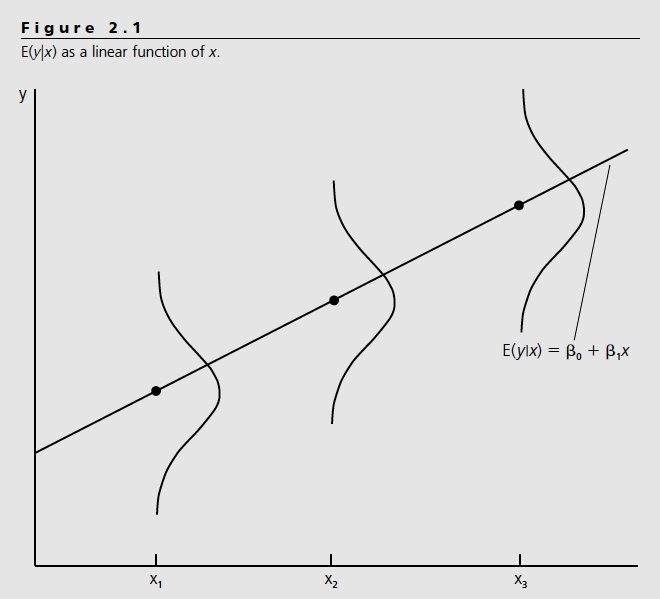
\includegraphics[scale=0.3]{fig1}
\end{center}

\end{frame}

%%------------------------------------------------------------------ %

\begin{frame}{Parâmetro Populacional (1)}

\begin{itemize}\itemsep1.2em

\item Vimos que: 

$$ E[x_i | u_i] = 0 \Longrightarrow  E[u_i] = 0 \text{ e } E[x_i u_i ] =0 $$

\item O termo de erro pode ser escrito como:

$$ u_i = y_i - \alpha - \beta x_i $$ 

\item Isso implica que: 

$$ E[y_i - \alpha - \beta x_i] = 0$$

$$ E[x_i (y_i - \alpha - \beta x_i)] = 0 $$

\item Podemos utilizar o sistema de equações acima para computar os parâmetros $(\alpha, \beta)$.

\end{itemize}

\end{frame}

%%------------------------------------------------------------------ %

\begin{frame}{Parâmetro Populacional (2)}

\begin{itemize}\itemsep1.2em

\item A primeira equação implica:

$$ \alpha = E[y_i] - \beta E[x_i] $$

\item A segunda equação implica:

$$ E[x_i y_i] - \alpha E[x_i] - \beta E [x_i^2] = 0 $$

\item Substituindo $\alpha$, temos:

$$ E[x_i y_i] - E[x_i] E[y_i] - \beta \left( E [x_i^2] - E[x_i]^2 \right) = 0 $$  

\item Portanto:

$$ \beta = \frac{E[x_i y_i] - E[x_i] E[y_i]}{E [x_i^2] - E[x_i]^2} = \frac{cov(x_i,y_i)}{var (x_i)} $$

\end{itemize}

\end{frame}

%------------------------------------------------------------------ %

\subsection{Estimação}

%------------------------------------------------------------------ %
    
\begin{frame}{Estimação (1)}

    \begin{itemize}\itemsep1.2em
    
     \item Na prática iremos estimar os parâmetros a partir de uma amostra $\left\{ (y_i, x_{i}): i=1,...n \right\}$.  
	 
	 \end{itemize}
	 
	 \centering
    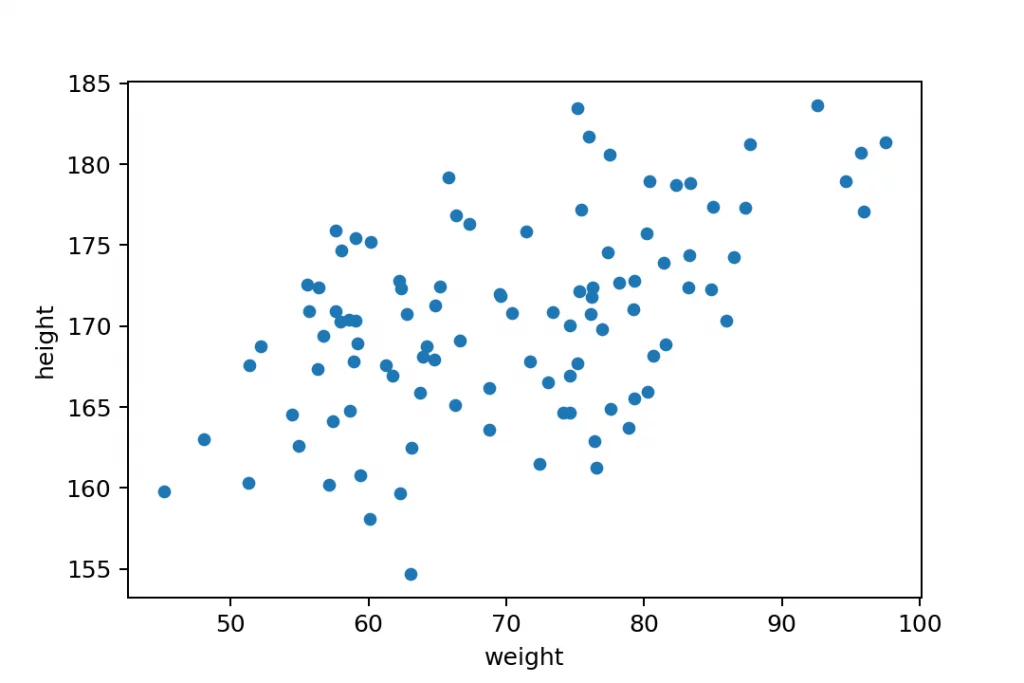
\includegraphics[height=0.7\textheight]{scatter}
    
\end{frame}

%------------------------------------------------------------------ %

\begin{frame}{Estimação (2)}

    \begin{itemize}\itemsep1.2em
    
     \item Na prática iremos estimar os parâmetros a partir de uma amostra $\left\{ (y_i, x_{i}): i=1,...n \right\}$. 
      
     \item Note que cada observação $i$ é uma retirada da população que segue a relação entre $y_i$ e $x_i$ do modelo populacional. 
     
     \item Portanto, o modelo amostral é:
     
     $$ y_i = \alpha + \beta x_i + u_i, \forall i = \left\{1,...,n \right\} $$
      
	 \item Como podemos estimar os parâmetros $(\hat{\alpha},\hat{\beta})$?
	 
	 \item É possível estimar esses parâmetros utilizando os análogos amostrais das condições $E[u_i] = 0$ e $E[x_i u_i ]=0$.  
	 
	 \end{itemize}
    
\end{frame}

%------------------------------------------------------------------ %

\begin{frame}{Estimação (3)}

    \begin{itemize}\itemsep1.2em
    
     \item Podemos utilizar os análogos amostrais das condições $E[u_i] = 0$ e $E[x_i u_i ]=$.
     
     $$ \frac{1}{n} \sum_{i=1}^n \left( y_i - \alpha - \beta x_i \right) = 0 $$
     
     $$  \frac{1}{n} \sum_{i=1}^n  \left[ x_i \left( y_i - \alpha - \beta x_i \right) \right] = 0 $$
     
     \item Resolvendo o sistema:
     
     $$ \hat{\alpha} = \overline{y} - \hat{\beta} \overline{x} $$
     
     $$ \hat{\beta} = \frac{\sum (y_i - \overline{y})(x_i - \overline{x})}{\sum (x_i - \overline{x})^2} = \frac{\widehat{cov(x_i,y_i)}}{\widehat{var (x_i)}} $$
     
     \end{itemize}
    
\end{frame}

%------------------------------------------------------------------ %

\begin{frame}{Estimação (4)}

    \begin{itemize}\itemsep1.2em
    
     \item O estimador obtido é chamado de estimador de \textbf{método dos momentos}.
     
     \item Esse nome decorre dele ser construído a partir de condições de momento (``médias'' que devem ser iguais a zero).
     
     \item Essas condições de momento decorrem diretamente das hipóteses do modelo de regressão linear, i.e., de hipóteses sobre o processo gerador de dados. 
     
     \item Essas hipóteses que garantem que $\hat{\beta}$ identifica o \textbf{efeito causal} de mudanças de $x$ sobre $y$. 
     
     \end{itemize}
    
\end{frame}

%------------------------------------------------------------------ %

\begin{frame}{Reta de Regressão (1)}

    \begin{itemize}\itemsep1.2em
    
     \item A reta de regressão é a reta que conecta $x$ com a expectativa condicional de $y$:
     
     $$ \hat{y}_i = \hat{\alpha} + \hat{\beta} x_i $$
     
     \item Os parâmetros $(\hat{\alpha},\hat{\beta})$ podem ser interpretados como o intercepto e a inclinação dessa reta de regressão. 
     
     \item Os resíduos podem ser definidos como a distância de cada observação para a reta de regressão:
     
     $$ \hat{u}_i = y_i - \hat{y}_i = y_i - \hat{\alpha} - \hat{\beta} x_i $$ 
     
     \end{itemize}
    
\end{frame}

%------------------------------------------------------------------ %

\begin{frame}{Reta de Regressão (2)}

	 \centering
    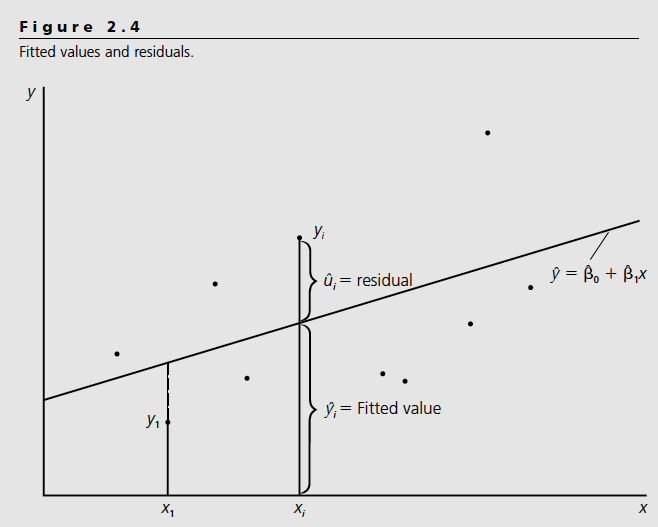
\includegraphics[height=0.8\textheight]{fig2}	
    
\end{frame}

%------------------------------------------------------------------ %

\begin{frame}{Mínimos Quadrados Ordinários (1)}

    \begin{itemize}\itemsep1.2em
    
     \item A reta de regressão nos dá uma outra intuição para os parâmetros $(\hat{\alpha},\hat{\beta})$. 
     
     \item Esses parâmetros constroem a reta mais bem ajustada ao conjunto de dados. 
     
     \item Formalmente, 
     
      $$ \underset{\alpha,\beta}{min} \sum_{i=1}^n u_i^2 =  \underset{\alpha,\beta}{min} \sum_{i=1}^n (y_i - \alpha - \beta x_i)^2 $$
      
      \item Os parâmetros minimizam isso significa que esses parâmetros são aqueles que minimizam uma métrica de distância entre valores observados e preditos.
     
     \end{itemize}
    
\end{frame}

%------------------------------------------------------------------ %

\begin{frame}{Mínimos Quadrados Ordinários (2)}

    \begin{itemize}\itemsep1.2em
    
     \item As condições de primeira ordem desse problema são:
     
     $$ \sum_{i=1}^n \left( y_i - \alpha - \beta x_i \right) = 0 $$
     
     $$ \sum_{i=1}^n  \left[ x_i \left( y_i - \alpha - \beta x_i \right) \right] = 0 $$
     
	\item O sistema de equações acima é exatamente o mesmo obtido utilizando método dos momentos.
	
	\item Solução é idêntica e resulta no mesmo intercepto e inclinação.        
     
     \end{itemize}
    
\end{frame}

%%------------------------------------------------------------------ %

\begin{frame}{Modelo de Regressão em R}

    \begin{itemize}\itemsep1.2em
    
     \item Estimaremos um modelo de regressão no R em três etapas: 
     
     \begin{enumerate}
     \item Simular um conjunto de dados. 
  
     \item Computar estimadores de mínimos quadrados ordinários manualmente. 
     
     \item Computar estimadores de mínimos quadrados ordinários utilizando funções do R.            
    
	\end{enumerate}          
     
	\item Utilizaremos o RStudio. 
     
     \end{itemize}
    
\end{frame}

%%------------------------------------------------------------------ %

\begin{frame}[fragile]
	\frametitle{Pacotes}

\vspace{0.5cm}
Começamos carregando um pacote para estimar regressões lineares.

\begin{lstlisting}

  # Instala pacote #	

    install.packages("estimatr")

  # Carrega pacote #  
      
	library(estimatr)
   
\end{lstlisting}

\end{frame}

%------------------------------------------------------------------ %

\begin{frame}[fragile]
	\frametitle{Coeficientes de MQO}
	
\vspace{0.5cm}

Considere uma amostra de 10.000 observações de um conjunto de dados cujo modelo populacional é dado por $y_i = 5.5*x_i + u_i$ em que  $x_i \sim N(0,1)$ e $u_i \sim N (0,100)$.  

\begin{lstlisting}

## Constroi vetores y, x e u ## 

set.seed(33)

x = rnorm(10000)

u = 10*rnorm(10000)

y = 5.5*x + u

## Estima parâmetros ##

beta = sum( (y- mean(y) )*(x - mean(x) ) ) / sum( (x-mean(x) )^2 )

alpha = mean(y) - beta*mean(x)   

\end{lstlisting}

\end{frame}

%------------------------------------------------------------------ %

\begin{frame}[fragile]
	\frametitle{Comando lm\_robust()}
	
\vspace{0.5cm}
Podemos utilizar o comando lm\_robust() para estimar regressões.

\begin{lstlisting}

## Comando lm_robust() ##

lm_robust(y ~ x)

## Objeto com resultados...

modelo = lm_robust(y ~ x)

## O que temos no objeto? 

modelo$coefficients # coeficientes #

modelo$vcov # matriz de variância #

\end{lstlisting}

\end{frame}

%------------------------------------------------------------------ %

\begin{frame}[fragile]
	\frametitle{Fit}
	
\begin{itemize}\itemsep1.2em 

\item A variância de $y$ pode ser decomposta em dois termos:

\begin{align*}
SQT &= \sum_{i=1}^n (y_i - \overline{y})^2 = \sum_{i=1}^n \left[ (y_i - \hat{y}_i) + (\hat{y}_i - \overline{y})\right]^2 \\
&= \sum_{i=1}^n u_i^2 + 2 \sum_{i=1}^n u_i (\hat{y}_i - \overline{y}) + \sum_{i=1}^n (\hat{y}_i - \overline{y})^2 \\
&=  \sum_{i=1}^n u_i^2 + \sum_{i=1}^n (\hat{y}_i - \overline{y})^2 \\
&= SQR + SQE
\end{align*}

\item Importância relativa de SQR e SQE é medida de ``ajuste'' da regressão.

\end{itemize}

\end{frame}

%------------------------------------------------------------------ %

\begin{frame}[fragile]
	\frametitle{Fit}
	
\begin{itemize}\itemsep1.2em 

\item Essa medida de ajuste é chamada de $R2$.

\item Ela é definida como:

$$ R2 = \frac{SQE}{SQT} = 1- \frac{SQR}{SQT}$$

\item Intuitivamente ela nos dá uma medida de quanto da variância de $y$ é explicado (no sentido estatístico) por $x$. 

\end{itemize}

\end{frame}

%------------------------------------------------------------------ %

\begin{frame}[fragile]
	\frametitle{Fit}
	
    \centering
    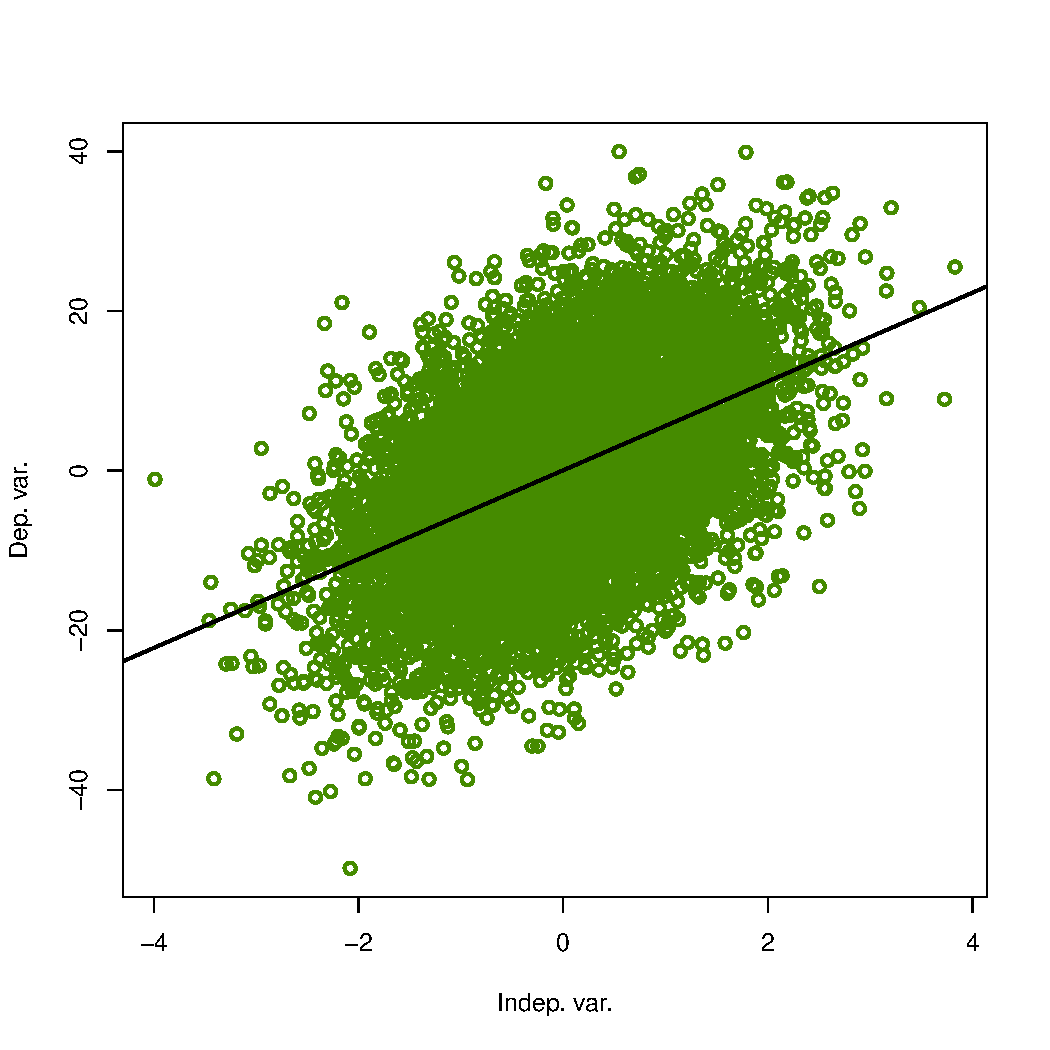
\includegraphics[height=\textheight]{fit}

\end{frame}

%------------------------------------------------------------------ %

\begin{frame}[fragile]
	\frametitle{Como eu fiz isso?}

\begin{lstlisting}

# inicio o arquivo onde vou salvar o grafico
pdf("fit.pdf")   

# faço gráfico dos dados utilizados na estimacao 
plot(x,y, type = "p", xlab = "Indep. var.", ylab = "Dep. var.", lwd = 2, col = "chartreuse4") 

# adiciono a linha com o y predito
abline(a = alpha, b = beta, lwd = 2, col = "black") 

# fecho o arquivo
dev.off()   

\end{lstlisting}

\end{frame}

%------------------------------------------------------------------ %

\begin{frame}[fragile]
	\frametitle{Fit}
	
\begin{itemize}\itemsep1.2em

\item O \textit{fit} não tem relação com a identificação dos parâmetros do modelo. 

\item A identificação depende apenas da expectativa do erro condicional ao regressor ser zero ($E[u_i|x_i]=0$).

\item O $R2$ se relaciona apenas com a proporção da variação em $y$ que é explicada por $x$ e que não é explicada por $x$ (``explicada'' por $u$).

\end{itemize}

\end{frame}

%------------------------------------------------------------------ %

\begin{frame}[fragile]
	\frametitle{$\beta$ idêntico, $R2$ diferente}

\begin{lstlisting}

# Modelo Original ##

y = 5.5*x + u 

summary(lm_robust(y ~ x))

Coefficients:
            Estimate Std. Error t value Pr(>|t|) CI Lower CI Upper   DF
(Intercept)   0.0474     0.1003  0.4725   0.6366  -0.1492    0.244 9998
x             5.5604     0.1018 54.6002   0.0000   5.3608    5.760 9998

Multiple R-squared:  0.2297 ,	Adjusted R-squared:  0.2296 

## Menos dispersão ##

y = 5.5*x + 0.1*u

summary(lm_robust(y ~ x))

Coefficients:
            Estimate Std. Error t value Pr(>|t|)    
(Intercept)  0.00474    0.01003   0.472    0.637    
x            5.50604    0.01018 540.664   <2e-16 ***
---
Multiple R-squared:  0.9669,	Adjusted R-squared:  0.9669 

\end{lstlisting}

\end{frame}

%------------------------------------------------------------------ %

\begin{frame}[fragile]
	\frametitle{Menos Dispersão}
	
    \centering
    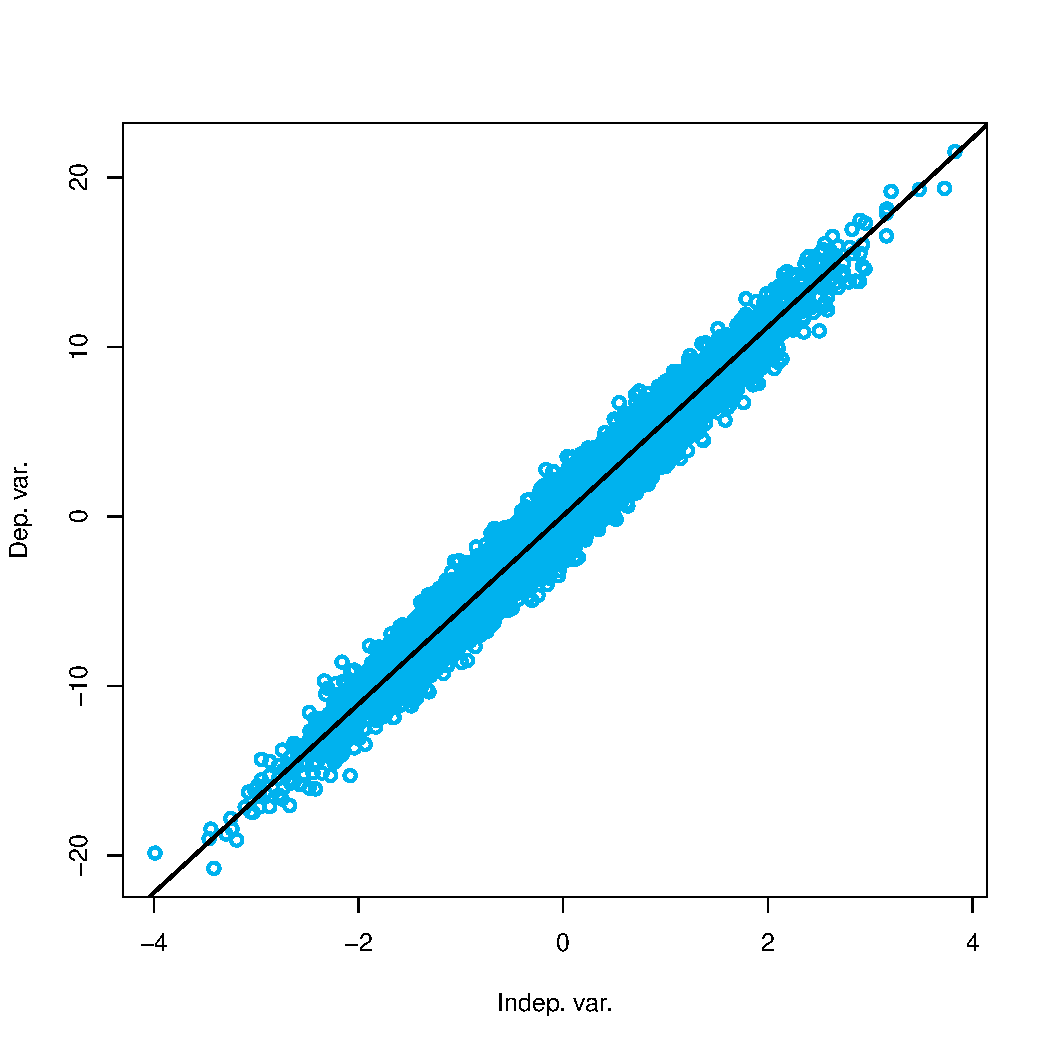
\includegraphics[height=\textheight]{fit_melhor}

\end{frame}

%------------------------------------------------------------------ %

\begin{frame}[fragile]
	\frametitle{Como eu fiz isso?}

\begin{lstlisting}

# inicio o arquivo onde vou salvar o grafico
pdf("fit.pdf")   

# faço gráfico dos dados utilizados na estimacao 
plot(x,y, type = "p", xlab = "Indep. var.", ylab = "Dep. var.", lwd = 2, col = "deepskyblue2") 

# adiciono a linha com o y predito
abline(a = alpha, b = beta, lwd = 2, col = "black") 

# fecho o arquivo
dev.off()   

\end{lstlisting}

\end{frame}

%------------------------------------------------------------------ %

\subsection{Interpretação}

%------------------------------------------------------------------ %

\begin{frame}{Interpretação de Coeficientes}

\begin{itemize}\itemsep1.2em

    \item Considere o modelo:
    
    $$ y_i = \alpha + \beta x_i + u_i $$
    
    \item Coeficiente $\beta$ nos dá o efeito de um aumento unitário em $x_i$. 
    
    \item Mas muitas vezes o interesse é em outras métricas.
    
    \item \textbf{Exemplos}:
    
    \begin{enumerate}
    \item Um aumento unitário em $x$ aumenta / diminui $y$ em quantos \%?
    \item Um aumento de 1\% em $x$ aumenta / diminui $y$ em quantos \%?
    \item Um aumento de um desvio-padrão de $x$ aumenta / diminui $y$ em quantos desvios-padrão?   
	\end{enumerate}     
    
	\item Duas alternativas: reescalonar coeficientes ou modificar modelo.     
    
    \end{itemize}

\end{frame}

%------------------------------------------------------------------ %

\begin{frame}{Modelo log-nível}

\begin{itemize}\itemsep1.2em

    \item Considere o modelo:
    
    $$ \log y_i = \alpha + \beta x_i + u_i $$
    
    \item Esse modelo implica:
    
    $$ y_i = \exp (\alpha + \beta x_i + u_i) $$
    
	\item O efeito de um aumento unitário de $x$ é:
	
	$$ \frac{\Delta y_i}{\Delta x_i} = \exp (\alpha + \beta (x_i + 1) + u_i) - \exp (\alpha + \beta x_i + u_i) = (\exp(\beta)-1) y_i $$      
    
    \end{itemize}

\end{frame}

%------------------------------------------------------------------ %

\begin{frame}{Modelo log-nível}

\begin{itemize}\itemsep1.2em
	
	\item Esse efeito como proporção de $y$ (``percentual'') é:
	
	$$ \frac{\Delta y_i}{\Delta x_i} \times \frac{1}{y_i} =  \exp(\beta)-1 \approx \beta $$   
    
    \item Portanto, o coeficiente desse modelo aproxima o efeito percentual de um aumento unitário de $x$. 
    
    \item Aproximação funciona mal quando coeficiente é grande (\textbf{regra de bolso}: acima de 0.3).       
    
    \end{itemize}

\end{frame}

%------------------------------------------------------------------ %

\begin{frame}{Modelo log-log}

\begin{itemize}\itemsep1.2em

    \item Considere o modelo:
    
    $$ \log y_i = \alpha + \beta \log x_i + u_i $$
    
    \item O coeficiente desse modelo identifica o efeito de um aumento de $\log x$ em $\log y$.     
    
    \item Sabemos que uma pequena no logaritmo de uma variável aproxima uma mudança percentual nessa variável.
    
    \item Portanto, o modelo identifica efeitos percentuais em $y$ de mudanças percentuais em $x$.
    \begin{itemize}
    \item Em economia esse parâmetro é tipicamente chamado de elasticidade.
    \end{itemize}
 
    \end{itemize}

\end{frame}

%------------------------------------------------------------------ %

\begin{frame}[fragile]
	\frametitle{Exemplo: educação e salários}

\vspace{0.5cm}

Iremos ilustrar questões relativas a forma funcional com dados reais.

\begin{lstlisting}

    root = ""

    setwd(root)
    
  # Instala e carrega pacote #
  
  	install.packages("tidyverse")
  	
  	library(tidyverse)    	
  	
  	library(haven)  
    
  # Abre banco de dados #  
    
    twins = read_dta("pubtwins.dta")
    
  # Resume variáveis do banco de dados #
  
  	summary(twins)

\end{lstlisting}

\end{frame}

%------------------------------------------------------------------ %

\begin{frame}[fragile]
	\frametitle{Modelo em nível}

\vspace{0.5cm}
Começando com uma regressão em nível.

\begin{lstlisting}

	mod = lm_robust(hrwage ~ educ, data = twins)
	
	summary(mod)
	
	Call:
lm_robust(formula = hrwage ~ educ, data = twins)

Standard error type:  HC2 

Coefficients:
            Estimate Std. Error t value  Pr(>|t|) CI Lower CI Upper  DF
(Intercept)  -12.705     3.5909  -3.538 4.306e-04  -19.756   -5.654 678
educ           1.935     0.2757   7.017 5.495e-12    1.393    2.476 678

Multiple R-squared:  0.09498 ,	Adjusted R-squared:  0.09364 
F-statistic: 49.24 on 1 and 678 DF,  p-value: 5.495e-12

\end{lstlisting}

\end{frame}

%------------------------------------------------------------------ %

\begin{frame}[fragile]
	\frametitle{Interpretação}

\begin{itemize}\itemsep1.2em

\item Um ano de estudo aumenta salário por hora em \$ 1.93. 

\item Qual o efeito percentual?  

\end{itemize}

\begin{lstlisting}

	mod$coefficients["educ"]/mean(twins$hrwage)
	
	0.1340074

\end{lstlisting}

\begin{itemize}\itemsep1.2em

\item Um ano de estudo aumenta salário por hora em cerca de 13\%.   

\end{itemize}

\end{frame}

%------------------------------------------------------------------ %

\begin{frame}[fragile]
	\frametitle{Modelo log-nível}

\vspace{0.5cm}
Rodamos agora uma regressão log-nível.

\begin{lstlisting}

	mod = lm_robust(lwage ~ educ, data = twins)
	
	summary(mod)
	
Call:
lm_robust(formula = lwage ~ educ, data = twins)

Standard error type:  HC2 

Coefficients:
            Estimate Std. Error t value  Pr(>|t|) CI Lower CI Upper  DF
(Intercept)   1.0077    0.15791   6.381 3.257e-10  0.69761   1.3177 678
educ          0.1022    0.01151   8.880 5.934e-18  0.07958   0.1248 678

Multiple R-squared:  0.1164 ,	Adjusted R-squared:  0.1151 
F-statistic: 78.86 on 1 and 678 DF,  p-value: < 2.2e-16

\end{lstlisting}

\end{frame}

%------------------------------------------------------------------ %

\begin{frame}[fragile]
	\frametitle{Interpretação}

\begin{itemize}\itemsep1.2em

\item Um ano de estudo aumenta salário por hora em torno de 10\%. 

\item Esse efeito é uma aproximação (efeito exato é $\exp(0.1022)-1 = 0.1076$).

\item Modelo em log diminui influência dos \textit{outliers} no resultado (mais sobre isso nas próximas aulas)  

\end{itemize}

\end{frame}

%------------------------------------------------------------------ %

\section{Modelo de Regressão Multivariado}

\subsection{Modelo Populacional}

%------------------------------------------------------------------ %

\begin{frame}{Modelo de Regressão Multivariado}

\begin{itemize}\itemsep1.2em

    \item Considere agora a relação populacional entre uma variável dependente ($y$) e um conjunto de regressores ($x_1,\cdots,x_k$) é:
    
    $$ y_i = \beta_1 x_{1i} + \beta_2 x_{2i} + ... + \beta_{k} x_{ki} + u_i = X_i' \beta + u_i, \, \forall i$$
    
\vspace*{0.2cm}     
    
    onde $i$ indexa a $i$-ésima observação da população
    
\vspace*{0.2cm}    
    
    $X_i$ é um vetor $k \times 1$ de regressores e $\beta$ é um vetor $k \times 1$ de parâmetros. 
    
\vspace*{0.2cm}     
    
    Normalmente a primeira linha de $X$ é uma constante.    
    
    \end{itemize}

\end{frame}

%------------------------------------------------------------------ %

\begin{frame}{Hipóteses (revisão)}

\begin{itemize}\itemsep1.2em 
	
	\item A hipótese fundamental é que $E[u_i | X_i] = 0$.
            
	\item \textbf{Implicação 1}: $E[u_i]=0$
	
	\vspace{0.3cm}
	
	\textit{Prova}: $E[u_i] = E \left[ E[u_i | X_i ] \right] = 0$  
	
	\item \textbf{Implicação 2}: $E[u_i X_i]=0$

\vspace{0.3cm}
	
	\textit{Prova}: $E[u_i X_i] = E \left[ E[u_i X_i | X_i ] \right] = E \left[ E[u_i  | X_i ] X_i \right] = 0$  
	
	\item Tipicamente supõe-se que $u_i \sim N(0, \sigma^2)$. Mas essa hipótese não é essencial.      
        
\end{itemize}

\end{frame}

%------------------------------------------------------------------ %

\begin{frame}{Interpretação (1)}

\begin{itemize}\itemsep1.2em 
	
	\item $\beta_k$ é efeito de uma mudança em $x_k$ sobre $y$ mantendo os outros regressores fixos
	
	\item Isso significa que modelo permite estudar efeito de mudar apenas um regressor mesmo quando dados incluem variação de todos eles ao mesmo tempo. 
	
	\item Tenta ``emular'' experimento controlado em que só um regressor é manipulado. 
        
\end{itemize}

\end{frame}

%------------------------------------------------------------------ %

\begin{frame}{Interpretação (2)}

\begin{itemize}\itemsep1.2em 
	
	\item Temos interesse no efeito de múltiplos regressores em $y$.
	
	\item \textbf{Modelo de preços hedônicos}:
	
	\begin{itemize}
		\item $p_i$ é o preço de um bem heterogêneo (ex.: carro) 
	
	\item $X_i$ é vetor de características observáveis desse bem (ex.: marca, potência, cor, tamanho etc.)
	
	\item Interesse em estimar o efeito de diferentes características sobre preço (``valoração''). 
		
	\end{itemize}
	
	\item Modelo de regressão multivariado conectando preço a diferentes características:
	
	$$ p_i = X_i' \beta + u_i $$ 
        
\end{itemize}

\end{frame}

%------------------------------------------------------------------ %

\begin{frame}{Interpretação (3)}

\begin{itemize}\itemsep1.2em 
	
	\item Temos interesse no efeito de um regressor $x_{i1}$ sobre $y$.
	
	\item Mas inserimos regressores adicionais para garantir que regressor não é correlacionado com termo de erro (``controles'').  
	
	\item Considere o modelo:
	
	$$ y_i = \beta_0 + \beta_1 x_{i1} + \varepsilon_i  = \beta_0 + \beta_1 x_{i1} + \beta_2 x_{i2} + u_i $$
	
	\item $x_{i1}$ correlacionado com termo de erro da primeira equação ($E[ x_{i1} \varepsilon_i ] \neq 0$).
	
	\item $x_{i1}$ não correlacionado com termo de erro da primeira equação ($E[ x_{i1} u_i ] = 0$).
        
\end{itemize}

\end{frame}

%------------------------------------------------------------------ %

\begin{frame}{Parâmetro Populacional (1)}

\begin{itemize}\itemsep1.2em
    
    \item Podemos utilizar $ E[X_i u_i ] = 0 $ para derivar o parâmetro populacional.
    
	\item Note que $u_i =   y_i - X_i' \beta$. Portanto,
	  
    $$ E[X_i u_i ] = E[X_i(y_i - X_i' \beta)] = E[X_i y_i] - E[X_i X_i'] \beta = 0 $$
    
    \item Isso implica que o parâmetro populacional é: 
    
    $$ \beta = E[X_i X_i']^{-1} E[X_i y_i] $$
    
    \item Lembre que $X_i$ é $k \times 1$ o que implica que $E [ X_i X_i' ]^{-1}$ tem dimensão $k \times k$ e $E[X_i y_i]$ dimensão $k \times 1$. 
    
    \item Logo, $\beta$ tem dimensão $k \times 1$ como gostaríamos.  
        
\end{itemize}

\end{frame}

%------------------------------------------------------------------ %

\begin{frame}{Parâmetro Populacional (2)}

\begin{itemize}\itemsep1.2em
    
    \item Note que $E[u_i |X_i ] = 0$ implica:
	
	$$ E [ y_i | X_i] = X_i \beta $$       
    
    \item Isso implica que $(y_i,X_i)$ tem distribuição normal bivariada se $u_i \sim N(0, \sigma^2)$.
	
	\item Em estatística aprendemos que sob normalidade conjunta $\beta$ é dado por $E[X_i X_i']^{-1} E[X_i y_i]$.
        
\end{itemize}

\end{frame}

%------------------------------------------------------------------ %

\subsection{Estimação}
    
%------------------------------------------------------------------ %    
    
\begin{frame}{Estimação (1)}

    \begin{itemize}\itemsep1.2em
    
      \item Suponha que queremos estimar os parâmetros do modelo de regressão linear a partir de uma amostra $\left\{ (y_i, x_{i1},…, x_{ik}): i=1,...n \right\}$. 
      
      \item Note que cada observação $i$ é uma retirada da população que segue a relação entre $y_i$ e $X_i$ do modelo populacional. 
      
      \item Logo, o modelo amostral pode ser escrito como:
        
        $$ {y = X \beta + u}, $$
        
    \end{itemize}
    \vspace{0.5cm}
        
     onde $ X = \begin{bmatrix} X_{1}' \\ \vdots \\ X_{n}' \end{bmatrix} = \begin{bmatrix} x_{11} & \cdots & x_{1k} \\
\vdots & \ddots & \vdots \\ x_{n1} & \cdots & x_{nk} \end{bmatrix}; Y = \begin{bmatrix}y_{1} \\ \vdots \\ y_{n} \end{bmatrix} ; u = \begin{bmatrix}u_{1} \\ \vdots \\ u_{n} \end{bmatrix} $
    
\end{frame}

%------------------------------------------------------------------ %
    
\begin{frame}{Estimação (2)}
    
     \begin{itemize}\itemsep1.2em           

     \item Estimador de mínimos quadrados ordinários (MQO) é o conjunto de $\beta$s que minimiza a soma do quadrado dos resíduos:
   \begin{align*}
\hat{\beta} = \underset{\beta}{\mathrm{argmin}} \; \sum_{i=1}^n u_i^2 = \underset{\beta}{\mathrm{argmin}} \; \sum_{i=1}^n (y_i-X_i'\beta)^2  
\end{align*}

     \item Condição de primeira ordem (use regra da cadeia):
     
     $$ \sum_{i=1}^n 2 X_i (y_i-X_i'\hat{\beta}) = 0 $$
     
     $$ \sum_{i=1}^n ( X_i y_i) - \sum_{i=1}^n ( X_i X_i' ) \hat{\beta} = 0 $$
     
     $$ \hat{\beta} = \left( \sum_{i=1}^n X_i X_i' \right)^{-1} \left( \sum_{i=1}^n  X_i y_i \right) $$
     
    \end{itemize}
    
\end{frame}

%------------------------------------------------------------------ %

\begin{frame}{Estimação (3)}
    
     \begin{itemize}\itemsep1.2em           

     \item Em notação matricial:
   \begin{align*}
\sum_{i=1}^n u_i^2 = u'u = (Y-X\beta)'(Y-X\beta)
\end{align*}

     \item Minimizando $u'u$:     

$$ - 2 X' Y + 2 X'X \hat{\beta} = 0 \Longrightarrow \hat{\beta} = (X'X)^{-1} (X'Y) $$
    
	\item Note que o estimador só existe se a matriz $X$ tem o posto cheio (i.e., é inversível).    
     
    \end{itemize}
    
\end{frame}

%------------------------------------------------------------------ %
    
\begin{frame}{Estimação (3)}
    
     \begin{itemize}\itemsep1.2em   
     
     \item Estimador equivalente é obtido se tentamos tornar condição $E[X_i u_i] = 0$ na amostra o mais próxima possível de zero (método dos momentos).
     
     $$ \frac{1}{n} \sum_{i=1}^n X_i (y_i-X_i' \hat{\beta}) = 0 $$
     
     $$ \hat{\beta} = \left( \sum_{i=1}^n X_i X_i' \right)^{-1} \left( \sum_{i=1}^n  X_i y_i \right) $$
     
     \item Estimador equivalente é obtido se maximizamos a chance de $u_i = y_i - X_i' \beta$ ser normal com média $0$ e variância $\sigma^2$ (máxima verossimilhança) 
     
    \end{itemize}
    
\end{frame}

%------------------------------------------------------------------ %

\begin{frame}[fragile]
	\frametitle{Exemplo: Dados de Educação e Salários}

\vspace{0.5cm}
Começando com uma regressão bivariada.

\begin{lstlisting}

  # Regressoes #
    
    modelo1 = lm_robust(lwage ~ educ, data = twins) # resultados armazenados em uma lista contendo diferentes objetos como: #

    # coeficientes #
    
    modelo1$coefficients 
    
    # matriz de variância #
    
    modelo1$vcov
  
    # ... #

\end{lstlisting}

Podemos adicionar controles.

\begin{lstlisting}

    modelo2 = lm_robust(lwage ~ educ + age + age2, data = twins) # é possível adicionar controles #
    
    summary(modelo2)
    
    modelo3 = lm_robust(lwage ~ educ + age + age2 + female + white, data = twins) # é possível adicionar controles #
    
    summary(modelo3)

\end{lstlisting}

\end{frame}

%------------------------------------------------------------------ %

\begin{frame}[fragile]
	\frametitle{Comando modelsummary()}

\vspace{0.5cm}
É possível exportar os resultados da regressão para tabelas de diferentes formatos.

\begin{lstlisting}

	# instala e carrega pacote #
	
	install.packages("modelsummary")
	
	library(modelsummary)	

    # podemos exportar resultados para tabela em formatos como "texto", "html" ou "latex" # 
    
	 modelos = list("MQO 1" = modelo1,
               		"MQO 2" = modelo2,
               		"MQO 3" = modelo3)

	modelsummary(modelos)
    
    # pode salvar como Markdown, Latex ou mesmo Word (instalar pacote ``flextable'') 

\end{lstlisting}

\end{frame}

%------------------------------------------------------------------ %

\begin{frame}{Interpretação (1)}
    
     \begin{itemize}\itemsep1.2em   
     
     \item Que controles queremos incluir?
     
     \item \textbf{Bons controles:}
     
     \begin{itemize}
     \item ``Explicam'' variável dependente (\textbf{regra de bolso:} sua inclusão aumenta o $R2$?);     
     
     \item Potencialmente correlacionados com regressor de interesse (mas não determinados por ele). 
     
     \end{itemize}
     
     \item \textbf{Controles ruins:}
     
     \item Não explicam variável dependente ou são muito correlacionados entre si;
     
     \item São ``endógenos'' (potencialmente determinados pelo regressor de interesse).
     
    \end{itemize}
    
\end{frame}

%------------------------------------------------------------------ %

\begin{frame}{Interpretação (2)}
    
     \begin{itemize}\itemsep1.2em   
     
     \item \textbf{Exemplo}: Considere o uma regressão conectando salários com educação:
     
     $$ \log y_i = \alpha + \beta e_i + W_i' \Gamma + u_i $$
     
     \item Que controles incluir em $X_i$? 
     \begin{itemize}
     \item Controles como idade, sexo, cor, estado civil, habilidade, onde reside etc. são bons controles
     \item Características do emprego são controles ruins (ex,: setor de atividade). 
     \end{itemize}     
     
    \end{itemize}
    
\end{frame}

%------------------------------------------------------------------ %

\subsection{Regressão Residual}

%------------------------------------------------------------------ %

\begin{frame}{O que os controles fazem? (1)}
    
     \begin{itemize}\itemsep1.2em   
     
     \item Controlar por uma variável é equivalente a limpar a variação das variáveis de interesse que vem dos controles. 
     
     \item É possível ver isso com a ideia de \textbf{regressão residual}. 
     
     \item Considere modelo de regressão:
     
     $$ y_i = \beta_0 + \beta_1 x_{i1} + \beta_2 x_{i2} + u_i $$
     
     \item É possível expressar $\beta_1$ e $\beta_2$ como: 
     
     $$ \widehat{\beta}_1 = \frac{\sum_{i=1}^n \widehat{r}_{i1} y_i}{\sum_{i=1}^n \widehat{r}_{i1}^2}$$       
     
     $$ \widehat{\beta}_2 = \frac{\sum_{i=1}^n \widehat{r}_{i2} y_i}{\sum_{i=1}^n \widehat{r}_{i2}^2}$$       
     
    \end{itemize}
    
\end{frame}

%------------------------------------------------------------------ %

\begin{frame}{O que os controles fazem? (2)}
    
     \begin{itemize}\itemsep1.2em   
     
     \item $r_{i1}$ e $r_{i2}$ são resíduos de regressões de $x_{1i}$ em $x_{2i}$ e $x_{2i}$ e $x_{1i}$, respectivamente. 
     
     \item Intuição é que ``controlar'' limpa a variação de $x_1$ ou $x_2$ que vem do outro fator. 
     
     \item Isso permite estimar efeitos de uma variável mantendo a outra fixa. 
     
    \end{itemize}
    
\end{frame}

%------------------------------------------------------------------ %

\begin{frame}{Exemplo}

\begin{itemize}\itemsep1.2em

\item Relação entre $y$ e os regressores $x_1$ e $x_2$ seja descrita pelo modelo populacional:

$$ y = \beta_0 + \beta_1 x_1 + \beta_2 x_2 + u $$

\item Relação entre $x_1$ e $x_2$ é descrita por:

$$ x_2 = \alpha x_1 + \nu $$

\item Suponha que os parâmetros populacionais sejam $\beta_0 = 0.1$, $\beta_1 = 0.6$, $\beta_2 = 0.4$ e $\alpha = 0.5$ e as distribuições $u \sim N(0,4)$, $\nu \sim N(0,16)$ e $x_1 \sim N(0,1)$.

\end{itemize}

\end{frame}

%------------------------------------------------------------------ %

\begin{frame}[fragile]
	\frametitle{Dados}

\vspace{0.5cm}
Simulo 10.000 observações dos vetores $u$, $\nu$, $x_1$, $x_2$ e $y$.

\begin{lstlisting}

  # Vetores # 
    
	set.seed(1985)
   
	beta0 = 0.1

	beta1 = 0.6
   
	beta2 = 0.4
 
	alpha = 0.5
   
	u = rnorm(10000, mean = 0, sd = 2)
 
	v = rnorm(10000, mean = 0, sd = 4)

	x1 = rnorm(10000, mean = 0, sd = 1)
 
	x2 = alpha*x1+v
 
	y = beta0 + beta1*x1 + beta2*x2 + u
  
	dados = data.frame(cbind(y,x1,x2))

\end{lstlisting}

\end{frame}

%------------------------------------------------------------------ %

\begin{frame}[fragile]
	\frametitle{Regressão Multivariada}

\vspace{0.5cm}
Rodo regressão longa.

\begin{lstlisting}

  # Regressão # 
    
	full.model = lm_robust(y ~ x1 + x2, data = dados)
	
	summary(full.model)

Standard error type:  HC1 

Coefficients:
            Estimate Std. Error t value   Pr(>|t|) CI Lower CI Upper   DF
(Intercept)  0.06576   0.019964   3.294  9.915e-04  0.02663   0.1049 9997
x1           0.61181   0.020065  30.491 2.504e-195  0.57248   0.6511 9997
x2           0.39489   0.005066  77.950  0.000e+00  0.38496   0.4048 9997

Multiple R-squared:  0.4366 ,	Adjusted R-squared:  0.4364 
F-statistic:  3858 on 2 and 9997 DF,  p-value: < 2.2e-16

\end{lstlisting}

\end{frame}

%------------------------------------------------------------------ %

\begin{frame}[fragile]
	\frametitle{Regressão Residual}

\vspace{0.5cm}
Rodo regressões entre os regressores.

\begin{lstlisting}

	res.reg1 = lm_robust(x1 ~ x2, data = dados)

	res.reg2 = lm_robust(x2 ~ x1, data = dados)
	
	dados$r1 = dados$x1 - res.reg1$fitted.values
	dados$r2 = dados$x2 - res.reg2$fitted.values

\end{lstlisting}

\end{frame}

%------------------------------------------------------------------ %

\begin{frame}[fragile]
	\frametitle{Regressão Residual}

\vspace{0.5cm}
Rodo regressões residuais.

\begin{lstlisting}

summary(lm_robust(y ~ r1, data = dados))

Call:
lm_robust(formula = y ~ r1, data = dados)

Standard error type:  HC2 

Coefficients:
            Estimate Std. Error t value   Pr(>|t|)   CI Lower CI Upper   DF
(Intercept)  0.04987    0.02590   1.926  5.415e-02 -0.0008902   0.1006 9998
r1           0.61181    0.02636  23.210 4.098e-116  0.5601380   0.6635 9998

Multiple R-squared:  0.05184 ,	Adjusted R-squared:  0.05175 
F-statistic: 538.7 on 1 and 9998 DF,  p-value: < 2.2e-16

\end{lstlisting}

\end{frame}

%------------------------------------------------------------------ %

\begin{frame}[fragile]
	\frametitle{Regressão Residual}

\vspace{0.5cm}
Rodo regressões residuais.

\begin{lstlisting}

summary(lm_robust(y ~ r2, data = dados))

Call:
lm_robust(formula = y ~ r2, data = dados)

Standard error type:  HC2 

Coefficients:
            Estimate Std. Error t value Pr(>|t|) CI Lower CI Upper   DF
(Intercept)  0.04987   0.021497    2.32  0.02037 0.007732  0.09201 9998
r2           0.39489   0.005439   72.60  0.00000 0.384224  0.40555 9998

Multiple R-squared:  0.3466 ,	Adjusted R-squared:  0.3465 
F-statistic:  5271 on 1 and 9998 DF,  p-value: < 2.2e-16

\end{lstlisting}

\end{frame}

%------------------------------------------------------------------ %

\section{Propriedades}

%------------------------------------------------------------------ %

\begin{frame}[fragile]
	\frametitle{Propriedades (1)}

\begin{itemize}\itemsep1.2em

\item \textbf{Mínimos Quadrados Ordinários (MQO)}: estimadores com propriedades desejáveis.

\item O que são propriedades desejáveis?
\begin{enumerate}
\item \textbf{Não viesado}: expectativa do estimador do parâmetro é igual ao parâmetro verdadeiro
\item \textbf{Eficiente}: variância do estimador é a menor possível     
\end{enumerate}        

\item Para ver essas propriedades iremos listar um conjunto de hipóteses.

\item Depois derivaremos a média e a variância do estimador. 

\end{itemize}

\end{frame}

%------------------------------------------------------------------ %

\begin{frame}[fragile]
	\frametitle{Propriedades}

\begin{itemize}\itemsep1.2em

\item \textbf{Hipóteses}:
\begin{enumerate}
\item \textbf{Modelo populacional:} o modelo populacional é
$$ y = X \beta;$$
\item \textbf{Amostragem aleatória:} $\left\{ (y_i, x_{i1},…, x_{ik}): i=1,...n \right\}$ é uma amostra independente e identicamente distribuída;
\item \textbf{Independência condicional}: $E[u | X ] = 0$;
\item \textbf{Variação em $X$:} $X = [X_1', \cdots X_n']'$ é matriz $n \times k$ com posto cheio;
\item \textbf{Homocedasticidade:} a variância o termo de erro é constante:
$$ V [u | X] = E [u u' | X] = \sigma^2 I $$ 
\end{enumerate}  

\item As hipóteses acima muitas vezes são chamadas de hipóteses de Gauss-Markov.
\begin{itemize}
\item Muitas vezes é adicionada a hipótese que $u | X \sim N(0, \sigma^2 I)$. 
\end{itemize}      

\end{itemize}

\end{frame}

%------------------------------------------------------------------ %

\begin{frame}[fragile]
	\frametitle{Média de $\widehat{\beta}$}

\begin{itemize}\itemsep1.2em

\item A média do estimador de MQO condicional a $X$ é

\begin{align*}
E [\widehat{\beta} | X] &= E \left[ (X'X)^{-1} X'y | X \right] \\
&= E \left[ (X'X)^{-1} X'(X \beta + u) | X \right] \\
&= \beta + (X'X)^{-1} X' E[u | X] \\ 
&= \beta 
\end{align*}

\item Lembre que $E[\widehat{\beta}] = E \left[E [\widehat{\beta} | X] \right]$.

\item Isso significa $E[\widehat{\beta}] = E \left[E [\widehat{\beta} | X] \right] = E[\beta]=\beta$.  

\item Logo, $\widehat{\beta}$ é um estimador não viesado de $\beta$.

\end{itemize}

\end{frame}

%------------------------------------------------------------------ %

\begin{frame}[fragile]
	\frametitle{Média de $\widehat{\beta}$ (bivariado)}

\begin{itemize}\itemsep1.2em

\item A média do estimador de MQO condicional a $x_i$ é

\begin{align*}
E [\widehat{\beta} | x_i] &= E \left[ \frac{\sum (x_i - \overline{x})(y_i - \overline{y})}{\sum (x_i - \overline{x})^2} | x_i \right] \\
&= E \left[ \frac{\sum (x_i - \overline{x})y_i}{\sum (x_i - \overline{x})^2} | x_i \right] - E \left[ \frac{\sum (x_i - \overline{x}) \overline{y}}{\sum (x_i - \overline{x})^2} | x_i \right] \\
&= E \left[ \frac{\sum (x_i - \overline{x}) (\alpha + \beta x_i + u_i) }{\sum (x_i - \overline{x})^2} | x_i \right] \\
&= \beta + E \left[ \frac{\sum (x_i - \overline{x}) u_i}{\sum (x_i - \overline{x})^2} | x_i \right] \\
&= \beta + \left[ \frac{\sum (x_i - \overline{x})}{\sum (x_i - \overline{x})^2} \right] E \left[ u_i | x_i \right] = \beta
\end{align*}

\item Isso significa $E[\widehat{\beta}] = E \left[E [\widehat{\beta} | x_i] \right] = E[\beta]=\beta$. 

\end{itemize}

\end{frame}

%------------------------------------------------------------------ %

\begin{frame}[fragile]
	\frametitle{Variância de $\widehat{\beta}$}

\begin{itemize}\itemsep1.2em

\item A variância de $\widehat{\beta}$ condicional a $X$ é:

\begin{align*}
V [\widehat{\beta} | X] &= E \left[ (\widehat{\beta} - \beta)(\widehat{\beta} - \beta)'| X \right] 
\end{align*}

\item Note que: 
\begin{align*}
& \widehat{\beta} = (X'X)^{-1} X'y = (X'X)^{-1} (X'X) \beta + (X'X)^{-1} X'u \\
& \Longrightarrow  \widehat{\beta} - \beta = (X'X)^{-1} X'u
\end{align*}

\item Portanto: 
\begin{align*}
V [\widehat{\beta} | X] &= E \left[ ((X'X)^{-1} X'u)((X'X)^{-1} X'u)'| X \right] \\
&= E \left[ (X'X)^{-1} X' uu' X (X'X)^{-1} | X \right] \\
&= (X'X)^{-1} X' E[u u'| X]  X (X'X)^{-1} \\
&= \sigma^2 (X'X)^{-1}
\end{align*}

\end{itemize}

\end{frame}

%------------------------------------------------------------------ %

\begin{frame}[fragile]
	\frametitle{Variância de $\widehat{\beta}$}

\begin{itemize}\itemsep1.2em

\item A lei da variância total diz: 

$$ V [\widehat{\beta} ] = E \left[ V[\widehat{\beta} | X ] \right] + V \left[ E[\widehat{\beta} | X] \right] $$

\item Temos: 

$$V \left[ E[\widehat{\beta} | X] \right] = V [ \beta] = 0$$

\item Logo, 

$$ V [\widehat{\beta} ] = E \left[ V[\widehat{\beta} | X ] \right] = \sigma^2 (X'X)^{-1}$$

\item Variância do estimador de MQO depende da variância do termo de erro (``variância residual de y'') e da variância dos regressores.

\end{itemize}

\end{frame}

%------------------------------------------------------------------ %

\begin{frame}[fragile]
	\frametitle{Variância de $\widehat{\beta}$ (bivariado)}

\begin{itemize}\itemsep1.2em

\item A variância de $\widehat{\beta}$ condicional a $x_i$ é:

\begin{align*}
V [\widehat{\beta} | x_i] = E \left[ (\widehat{\beta} - \beta)^2 | x_i \right] 
\end{align*}

\item Note que: 
\begin{align*}
& \widehat{\beta} = \frac{\sum_{i=1}^n (x_i - \overline{x}) (y_i - \overline{y})}{\sum_{i=1}^n (x_i- \overline{x})^2} = \beta + \frac{\sum_{i=1}^n (x_i- \overline{x}) u_i}{\sum_{i=1}^n (x_i- \overline{x})^2} \\
& \Longrightarrow  \widehat{\beta} - \beta = \frac{\sum_{i=1}^n (x_i - \overline{x}) u_i}{\sum_{i=1}^n (x_i- \overline{x})^2} = \sum_{i=1}^n w_i u_i
\end{align*}

\item Portanto: 
\begin{align*}
V [\widehat{\beta} | x_i] &= E \left[ \left( \sum_{i=1}^n w_i u_i \right)^2 | x_i \right] = E \left[ \left( \sum_{i=1}^n w_i^2 u_i^2 \right) | x_i \right] \\
&=  \sigma^2 \left(\sum_{i=1}^n w_i\right)^2 = \frac{\sigma^2}{\sum_{i=1}^n (x_i- \overline{x})^2} 
\end{align*}

\end{itemize}

\end{frame}

%------------------------------------------------------------------ %

\begin{frame}[fragile]
	\frametitle{Teorema de Gauss-Markov}

\begin{itemize}\itemsep1.2em

\item Se as hipóteses 1-5 são válidas, o estimador de MQO é o melhor estimador linear não viesado do vetor $\beta$.

\item O que isso significa? Considere a classe de estimadores lineares:

$$ \widetilde{\beta} = \sum_{i=1}^n W_i y_i, $$

em que $W_i$ é uma função da amostra.

\item Teorema de Gauss-Markov diz que $W_i = (X_i X_i')^-1 X_i$ é a função que:
\begin{enumerate}
\item ... faz com que $\widetilde{\beta}$ tenha a menor variância possível (``melhor'')
\item ... entre os estimadores  que $E[\widetilde{\beta}] = \beta$ (``não viesado'')   
\end{enumerate}      

\end{itemize}

\end{frame}

%------------------------------------------------------------------ %

\begin{frame}[fragile]
	\frametitle{Distribuição Normal}

\begin{itemize}\itemsep1.2em

\item \textbf{Hipótese adicional}:

$$u | X \sim N(0, \sigma^2 I)$$     

\item Essa hipótese adicional caracteriza o que chamamos de \textbf{modelo de regressão linear clássico}.

\item Ela implica que o estimador $\widehat{\beta}$ tem distribuição normal.

\item \textbf{Por quê?} 

\begin{align*}
& \widehat{\beta} = \beta + (X'X)^{-1} X'u \\
& u | X \sim N(0, \sigma^2 I) \Longrightarrow \widehat{\beta} \sim N(\beta, \sigma^2 (X'X)^{-1})
\end{align*}

\end{itemize}

\end{frame}

%------------------------------------------------------------------ %

\end{document}

